\chapter{Corpus Preparation}
\label{chap:corpus}
  An expressive performance corpus is a set of performance samples. Since this research is based on a supervised learning algorithm, a high-quality corpus is essential to our success. Each sample consists of a score and its corresponding human recording. Some metadata such as structure analysis, harmonic analysis etc. may also be included. In this chapter, we will review some the existing corpora, specifications and formats of our corpus, and how we actually construct it.

\section{Existing Corpora} 
Unlike other research fields like speech processing or natural language processing, there exist virtually no public accessible corpus for computer expressive performance. CrestMusePEDB\cite{crestmuse} (PEDB stands for "Performance Expression Database") is a corpus created by Japan Science and Technology Agency's CREST program, however, until the time of this writing, we can't establish any contact with the database administrators. They use a graphical interface to annotate the expressive performance parameters from audio recordings.The repertoire covers many piano works from well-known classical composers like Bach, Mozart, and Chopin, and the recordings are from famous pianists. From their website\cite{crestmuse}they claim to contain the following data: PEDB-SCR - score text information, PEDB-DEV - performance deviation data and PEDB-IDX - audio performance credit. But the quality of the data is unknown.

Another example is the Magaloff Project\cite{magaloff}, which is a joint effort of some universities in Austria.  They invite Russian pianist Nikita Magaloff to record all solo works for piano by Frederic Chopin on a Bösendorfer SE computer-controlled grand piano. This corpus became the material for many subsequent researches \cite{Goebl2009, Grachten2011, Flossmann2009, Grachten2012, Flossmann2013, Flossman2011, Flossmann2010a}. Flossmann et al., one of the leading researchers of the project, also won the 2008 RenCon contest with a expressive performance system call YQX\cite{yqx} based on this corpus. However, the corpus is not opened up to the public. 

Since both corpora are not available, we need to implement our own one. We will start by defining the specification.

\section{Corpus Specification}

The corpus we need must fulfill the following constrains:
\begin{enumerate}
   \item All the samples are monophonic, containing only a single melody without chords.
   \item No human error, such as insertion, deletion, or wrong pitch exist in the recording; the score and recording are matched note-to-note.
   \item Phrasing is annotated by human. 
   \item The score, recording and phrasing data are in machine-readable format.

   %\item The tempo label in MIDI recordings are the tempo by which the musician played. 
\end{enumerate}

Some useful information are excluded because they are less relevant to our system. Examples are:

\begin{enumerate}
   \item Advanced Structural Analysis, such as GTTM (Generative Theory of Tonal Music)\cite{GTTM}
   \item Harmonic Analysis
   \item Instrument specific techniques, such as violin pizzicato, tapping, or bow techniques.
   \item Piano paddle usage
   \item Other instrument specific instructions, such as piano fingering, violin bow techniques etc.
\end{enumerate}

We choose Clementi's Sonatina Op. 36 for our corpus, because it is a must-learn repertoire for every piano student (especially in Asia), so it's easy to find a wide skill range of performers to record the corpus. These sonatina are in classical style, so the learned model be easily extended to other classical era works like Mozart or Haydn. There are six sonatinas included in Op. 36, the first five have three movements each, and the last one has two movements. The titles, tempo markers and time signatures of all the pieces are listed in Table \ref{tab:cleminfo}

\begin{table}
   \centering
   \caption{Clementi's Sonatinas Op. 36 }
   \label{tab:cleminfo}
   \begin{tabular}{lll}
      \hline
      \textbf{Title} & \textbf{Movement} & \textbf{Time Signature}\\
      \hline
      No. 1 Sonatina in C major&    I. Allegro &4/4\\
      &    II. Andante &3/4\\
      &    III. Vivace &3/8\\
      No. 2 Sonatina in G major&    I. Allegretto &2/4\\
      &    II. Allegretto &3/4\\
      &    III. Allegro &3/8\\
      No. 3 Sonatina in C major&    I. Spiritoso &4/4\\
      &    II. Un poco adagio &2/2\\
      &    III. Allegro &2/4\\
      No. 4 Sonatina in F major&    I. Con spirito &3/4\\
      &    II. Andante con espressione &2/4\\
      &    III. Rondó: Allegro vivace &2/4\\
      No. 5 Sonatina in G major&    I. Presto &2/2\\
      &    II. Allegretto moderato &3/8\\
      &    III. Rondó: Allegro molto &2/4\\
      No. 6 Sonatina in D major&    I. Allegro con spirito &4/4\\
      &   II. Allegretto   &6/8\\
      \hline
   \end{tabular}
\end{table}


 %we choose  for score to choose from, such as MusicXML\cite{Good2001}, LilyPond\cite{LilyPond}, Finale, Sibelius, ABC, MuseData, and Humdrum. The book \cite{Selfridge-Field1997} has a comprehensive review on this issue. %For research purpose, proprietary format like Finale and Sibelius is abandoned because of their limited support from open source tools. 
To represent Clemetni's work in digital format, we choose MusicXML. MusicXML is a digital score notation using XML (eXtensible Markup Language) , it can express most traditional music notations and metadata. Most music notation software and software tool supports musicXML format. An example snippet of a musicXML score is shown in Fig. \ref{fig:expxml}%LilyPond is a \LaTeX-like language for music typesetting. %ABC, MuseData and Humdrum are based on ASCII codes and each defines their unique representation for music score. 
\begin{figure*}[tp]
   \begin{center}
      %TODO:Fig.:Example JSON code
      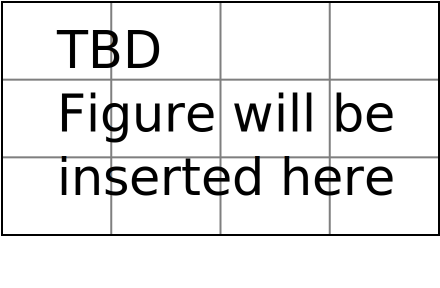
\includegraphics[width=\textwidth]{fig/TBDFigure}

   \end{center}
   \caption{Example MusicXML score}
   \label{fig:expxml}
\end{figure*}
%TODO: guitar pro?
Although MIDI is also a popular candidate for score representation in computer music research, it is designed to hold instrument control signal rather than notation. Some music symbols may not be available in MIDI. Furthermore, MIDI represents music as a series of note-on and note-off events, which requires additional effort to transform into traditional notation.

But for performance, MIDI is the most suitable format. Using a pressure sensitive digital piano, pianist can record in a natural way. The recordings have high precision in time and pitch, and polyphonic tracks can easily be separated. Although WAV (Waveform Audio Format) audio recording has higher fidelity than MIDI, but they are harder to parse by computers. Without robust onset detection, pitch detection, and source separation, the information is extremely difficult to extract.  Manually annotate each WAV recording takes a lot of manpower, and the accuracy may not be consistent. 

There's a way to keep both the score and the recording in one single MIDI file. Instead of recording the actual note-on and note-off timing, we keep the nominal note-on and note-off the same as in score. Then, MIDI tempo-change events are inserted before each note to shift the actual timing of the recorded notes. But since MIDI is so limited to represent a score, and it requires complex calculations to recover the performance from fixed notes and tempo-change events, this method is not used in the research.
%A human musician can't play every note exactly on the beat, even if playing along with a metronome. There are two ways to record this behavior: first, record the exact note-on and note-off time, while keeping the tempo fixed; second, keep the notes on the beat, so the MIDI looks the same as the score. Then insert tempo-change event between each notes, so notes of the same length can be rendered differently because they have different tempo marker. The second method may look smart, because the score and performance can be stored in one MIDI file instead of two, but it would involve complex calculation when linearly scaling the tempo. Since tempos from different samples need to be normalized during feature extraction, the first method is superior  than the second.
%Other formats such as image files (scanned or typesetted by computer) or PDF files are an alternative, but they are not an option for direct computer analysis. 

%In this research, we use MusicXML as the main vehicle for music score, because of the following reasons: first, it covers most music notations and metadata need for this research. Second, it is supported in most music notation software, including the one used in this research -- MuseScore. Finally, the music21 toolbox can convert many other formats into MusicXML without problem.

Finally, we store the phrasing, which is the only metadata we used, in a plaintext file, each line in the phrasing file is the starting point of each phrase. The starting point is defined as the onset timing (in quarter notes) from the beginning of the piece\footnote{For a phrase that start at a point which is a circulating decimal, for example $\frac{1}{3}$, the starting point can be alternatively defined as any finite decimal between the end of the last phrase and the start of the current phrase. For example, if the last phrase stops at beat 1, the second phrase start at $2\frac{1/3}=2.333\cdots$ beat, the start point of the second phrase can be written as 2.3 or 2.0, etc.} The phrasing is assigned by the us using the following criteria:, 
\begin{enumerate}
   \item Phrase may be separated by a salient pause.
   \item Phrase may end with a cadence.
   \item Phrase may be separated by dramatic change in tempo, key or loudness
   \item Repeated structures in tempo or pitch may be a phrase.
\end{enumerate}
The above criteria are just general principles, not strict rules, the phrasing is still decided subjectively.

   An automatic phrasing algorithm may be achieved in the future, either by fuzzy rules or by machine learning. With the automatic phrasing capability, the system can become fully automatic. But phrasing controls the structural expression of a piece, we left the phrasing decision to the user. Because we intend to leave some degree of freedom for users to expressive themselves. But note-level expression is too trivial to be assigned by hand, but deciding phrase-level expression is less demanding for an ordinary user. 

 
%\section{File Format}
\section{Implementation}

\subsection{Score Preparation}

The digital scores are downloaded from KernScore website \cite{KernScores}. The  scores are transformed into MusicXML from th original Hundrum file format (.krn) using the  music21 toolkit. Because this research focus on monophonic melody only, the accompaniments are remove and the chords are reduced to their highest-pitched note, which is usually the most salient melody line. The reduced scores are doubled-checked against a printed version publish by Durand \& Cie.,Paris \cite{Clementi1915} to eliminate all errors. %We use MuseScore notation editor to view and edit MusicXML; some metadata errors are corrected by editing the MusicXML with text editors .

\subsection{MIDI Recording}
We have implemented two methods for recording: First, using a Yamaha digital piano to record MIDI. Second, by tapping on a touch sensitive device to express tempo, duration and loudness. Due to accuracy consideration, only the recordings from Yamaha digital piano are selected.


We used a Yamaha P80 88-key graded hammer effect\footnote{Graded Hammer Effect feature provides realistic key pressure response similar to a traditional acoustic piano}digital piano for recording. Using a MIDI-to-USB converter, the keyboard is connected to Rosegarden Digital Audio Workstation (DAW) software on a Linux computer. The Rosegarden DAW also generated the metronome sound to help the performer maintain a steady speed. Metronome is mandatory because if the performer plays freely, the tempo information written in the MIDI file will be invalid, which makes subsequent parsing and linear scaling very difficult. So the performers are asked to follow the speed of the metronome, but they can apply any level of rubato they like. 

The second method, which is not used in the final experiments, is to utilize touch-enabled input device like smartphone touchscreen or laptop touchpad. We have implemented an prototype using a Synaptics Touchpad on a Lenovo ThinkPad X200i laptop. When the user taps the touchpad, one note from a predefined score will be played, the duration and loudness will be controlled by the time and pressure of the tap. So the user can \enquote{play} the touchpad like a musical instrument. This idea has already be used in musical games like Magic Piano \cite{magicpiano}. This method requires minimal instrument skill and utilize widely available hardware. But the accuracy in pressure is not satisfying, because most touchpad use contact area to estimate pressure. But it is indeed a low cost alternative toa MIDI digital piano.

\subsection{MIDI Cleaning and Phrase Splitting}
  After the MIDIs are recorded, we use scripts to check if each recording is matched note-to-note with its corresponding score. If not, the mistakes are manually corrected. %For example, if the pitch was played wrongly, we will correct the pitch but keep the onset, duration  and intensity as is. 
  If there are a small segments that is totally messed up, it will be reconstruct using repeated or similar segments from the same piece. The matched score and MIDI pair are then split into phrases according to the phrasing file. The split phrases are checked again for note-to-note match before they are used.

\section{Results}
Six graduate students (not majored in music) with varying piano skill are invited to record the samples. The number of mistakes they made are listed in Table \ref{tab:mistakes}. These mistakes are indetified using the unix \texttt{diff}\cite{diff} tool. Five of them (A to E) finished Clementi's entire Op. 36, perfomer F only recorded part of the work. The total number of recordings and the corresponding phrases/notes counts are shown in Table \ref{tab:corpuscount}. 
\framebox{TODO:mistakes}

\begin{sidewaystable}[bp]
   \centering
   \caption{Number of Mistakes in Corpus}
   \label{tab:mistakes}
   \begin{tabular}{crrrrrrrrrrrrrrrrr|r}
      \hline
      Performer&1-1&1-2&1-3&2-1&2-2&2-3&3-1&3-2&3-3&4-1&4-2&4-3&5-1&5-2&5-3&6-1&6-2&Subtotal\\
      \hline
      A&0&5&2&4&3&0&4&2&2&4&5&9&9&2&3&4&1&59\\
      B&2&1&1&2&2&1&6&0&3&2&3&6&12&3&3&10&7&64\\
      C&1&1&0&1&0&1&2&0&0&3&2&3&10&1&35&6&1&67\\
      D&0&1&1&2&3&1&4&1&1&10&6&3&10&2&7&13&2&67\\
      E&2&3&4&4&0&3&4&0&0&21&6&22&23&3&9&18&13&135\\
      F&1&3&2&11&6&8&7&2&6&&15&&&&20&&&81\\
      \hline
      Subtotal&6&14&10&24&14&14&27&5&12&40&37&43&64&11&77&51&24&473\\
   \end{tabular}
\end{sidewaystable}
\begin{table}[bp]
   \centering
   \caption{Total Recorded Phrases and Notes Count}
   \label{tab:corpuscount}
   \begin{tabular}{lrrr}
      \hline
      \bf Title&\bf Recordings&\bf Total Phrases&\bf Total Notes\\
      &\bf Count&&\\
      \hline
      No. 1 Mov. I&6&72&1332\\
      No. 1 Mov. II&6&60&882\\
      No. 1 Mov. III&6&102&1566\\
      No. 2 Mov. I&6&108&1920\\
      No. 2 Mov. II&6&36&750\\
      No. 2 Mov. III&6&168&2484\\
      No. 3 Mov. I&6&156&3156\\
      No. 3 Mov. II&6&42&444\\
      No. 3 Mov. III&6&120&2628\\
      No. 4 Mov. I&5&80&2325\\
      No. 4 Mov. II&6&78&1332\\
      No. 4 Mov. III&5&85&1920\\
      No. 5 Mov. I&5&85&3360\\
      No. 5 Mov. II&5&70&1580\\
      No. 5 Mov. III&6&144&3384\\
      No. 6 Mov. I&5&145&4180\\
      No. 6 Mov. II&6&78&2754\\
      \hline
      Total&97&1629&35997\\
      \hline
   \end{tabular}
\end{table}

The number of phrases (according to our phrasing) and notes are shown in Table \ref{tab:clemcount}. Fig. \ref{fig:notes} shows the length distribution of each movement, most movements are around a few hundred notes, except the long No.6 and some short second movements.  Fig. \ref{fig:phrases} shows the length distribution in numbers of phrases, most movements are around 20 phrases. The length distribution of the phrases in all six pieces are shown in Fig. \ref{fig:phrlength}, most phrases are shorter than 30 notes. Some very long phrases exists, they are often virtuoso segments with very fast note sequences, so they are hard to be further split.

\begin{table}[bp]
   \centering
   \caption{Phrases and Notes Count for Clementi's Sonatina Op. 36}
   \label{tab:clemcount}
   \begin{tabular}{lrr}
      \hline
      \textbf{Title}&\textbf{Phrases Count}&\textbf{Notes Count}\\
      \hline
      No. 1 Mov. I&12&222\\
      No. 1 Mov. II&10&147\\
      No. 1 Mov. III&16&261\\
      No. 2 Mov. I&18&320\\
      No. 2 Mov. II&6&125\\
      No. 2 Mov. III&28&414\\
      No. 3 Mov. I&25&526\\
      No. 3 Mov. II&6&74\\
      No. 3 Mov. III&19&438\\
      No. 4 Mov. I&25&465\\
      No. 4 Mov. II&12&222\\
      No. 4 Mov. III&16&384\\
      No. 5 Mov. I&17&672\\
      No. 5 Mov. II&13&316\\
      No. 5 Mov. III&24&564\\
      No. 6 Mov. I&28&836\\
      No. 6 Mov. II&11&459\\
      \hline
      \textbf{Total} &286&6445\\
      \hline
   \end{tabular}
\end{table}


\begin{figure*}[tp]
   \begin{center}
      \includegraphics[width=\textwidth]{fig/notes}

   \end{center}
   \caption{Movements Length (in Notes) Distribution}
   \label{fig:notes}
\end{figure*}
\begin{figure*}[tp]
   \begin{center}
      \includegraphics[width=\textwidth]{fig/phrases}

   \end{center}
   \caption{Movements Length (in Phrases) Distribution}
   \label{fig:phrases}
\end{figure*}

\begin{figure*}[tp]
   \begin{center}
      \includegraphics[width=\textwidth]{fig/phrlength}

   \end{center}
   \caption{Phrase Length (in Notes) Distribution}
   \label{fig:phrlength}
\end{figure*}






 %TODO:recording example pic
\framebox{TODO:mention Fig. \ref{fig:exprecording}}
\begin{figure*}[tp]
   \begin{center}
      %TODO:Fig.:Example JSON code
      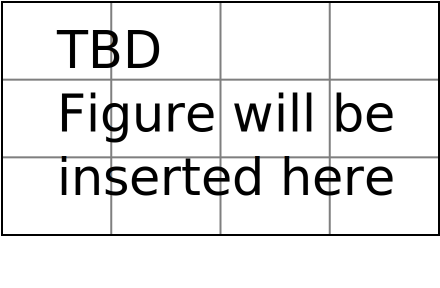
\includegraphics[width=\textwidth]{fig/TBDFigure}

   \end{center}
   \caption{Example Recording Compared to Score (Pianoroll)}
   \label{fig:exprecording}
\end{figure*}
\framebox{TODO:error count}

\framebox{REVIEW1}
